\documentclass[a4paper,11pt]{scrartcl}

\usepackage[ngerman]{babel}
% uncomment or modify according to your operating system
% \usepackage[applemac]{inputenc} % european characters can be used (Mac OS)
%\usepackage[latin1]{inputenc} 
%\usepackage{ucs} % fuer deutsche Sonderzeichen unter Linux
%\usepackage[utf8x]{inputenc} %fuer deutsche Sonderzeichen unter Linux
\usepackage[utf8]{inputenc} %fuer deutsche Sonderzeichen unter Windows
\usepackage[T1]{fontenc}
\usepackage{graphicx} 
\usepackage{fullpage}
\usepackage{latexsym}
\usepackage{amssymb}
\usepackage{amsmath}
\usepackage{ifthen}
\usepackage{listings}
\usepackage{color}
\usepackage{hyperref}
\usepackage{cite}

\definecolor{dkgreen}{rgb}{0,0.6,0}
\definecolor{gray}{rgb}{0.5,0.5,0.5}
\definecolor{mauve}{rgb}{0.58,0,0.82}
\lstset{ %
  language=Matlab,                % the language of the code
  basicstyle=\small,              % the size of the fonts that are used for the code
  numbers=left,                   % where to put the line-numbers
  numberstyle=\tiny\color{gray},  % the style that is used for the line-numbers
  stepnumber=1,                   % the step between two line-numbers. If it's 1, each line 
                                  % will be numbered
  numbersep=5pt,                  % how far the line-numbers are from the code
  backgroundcolor=\color{white},      % choose the background color. You must add \usepackage{color}
  showspaces=false,               % show spaces adding particular underscores
  showstringspaces=false,         % underline spaces within strings
  showtabs=false,                 % show tabs within strings adding particular underscores
  frame=single,                   % adds a frame around the code
  rulecolor=\color{black},        % if not set, the frame-color may be changed on line-breaks within not-black text (e.g. commens (green here))
  tabsize=2,                      % sets default tabsize to 2 spaces
  captionpos=b,                   % sets the caption-position to bottom
  breaklines=true,                % sets automatic line breaking
  breakatwhitespace=false,        % sets if automatic breaks should only happen at whitespace
  title=\lstname,                   % show the filename of files included with \lstinputlisting;
                                   % also try caption instead of title
  keywordstyle=\color{blue},          % keyword style
  commentstyle=\color{dkgreen},       % comment style
  stringstyle=\color{mauve},         % string literal style
  escapeinside={\%*}{*)},            % if you want to add LaTeX within your code
  morekeywords={end,sortrows}               % if you want to add more keywords to the set
}


% Abkuerzungen fuer haeufige Befehle wie z.B. griechische Buchstaben
\newcommand{\N}{\mathbb{N}}
\newcommand{\Z}{\mathbb{Z}}
\newcommand{\R}{\mathbb{R}}
\newcommand{\C}{\mathbb{C}}
\newcommand{\F}{\mathcal{F}}
\newcommand{\La}{\mathcal{L}}
\newcommand{\de}{\delta}
\newcommand{\e}{\varepsilon}
\newcommand{\la}{\lambda} 
\newcommand{\p}{\varphi} 
\newcommand{\al}{\alpha} 
\newcommand{\be}{\beta} 
\newcommand{\om}{\omega}
\newcommand{\Om}{\Omega}
\newcommand{\ta}{\tau}
\newcommand{\g}{\gamma}
\newcommand{\HE}{\mathbb{H}}
\newcommand{\E}{\mathbb{E}}
\newcommand{\vG}{\varGamma}
\newcommand{\s}{\sigma}

\begin{document}

\subject{LVA-Modeling and Simulation}
\title{Projecttitle}

\publishers{Supervisor: Max Mustermann}
\author{Marianne Musterfrau, Matricular Number - Curriculum Number\footnote{Created the results for case study 3 and wrote Chapter 2 of the documentation.}\\
Max Mustermann jun.,Matricular Number - Curriculum Number\footnote{Collected the data and wrote Chapter 3 of the documentation.}\\
Max Mustermann sen., Matricular Number - Curriculum Number\footnote{Implemented the base source code and evaluated case studies 1 and 2.}\\
Marianne Musterfrau sen., Matricular Number - Curriculum Number\footnote{Wrote introduction and discussion.}}

\maketitle

\begin{abstract}
Poorly written documentations of modelling projects are responsible for countless poor grades at Austrian universities. With this template, including the template abstract you are currently reading, we aim to reduce number of bad grades and improve the quality of scientific project documentations sustainably.
\end{abstract}

\newpage

\tableofcontents

\newpage

\section{Introduction}
\paragraph{Motivation.} 
Poorly written documentations of modelling projects are responsible for countless poor grades at Austrian universities. 
\paragraph{Introduction to the Topic.} The main causes range from poor structure to unscientific wording and typesetting.
\paragraph{Reated Work.} This problem has also been addressed by \cite{zeigler2000theory}, for example, but it differs greatly from the current project. Note, that literature must be inserted into File \textit{references.bib} and can be cited via \verb|\cite{QUELLE}|.
\paragraph{Aim.} However, goal of this project is to reduce this problem with the help of a template.

\section{Model}
\subsection{Modelling}
\label{sec:modelling}
We first describe the conceptual modeling. Hereby we may apply various types of formulas such as numbered equations, like
\begin{equation}
\label{eq:pythogoras}
 a^2 + b^2 = c^2,
\end{equation}
or non-numbered equations like
\begin{equation*}
 \al + \be + \g = 180.
\end{equation*}
Numberes equations can be referenced via (\ref{eq:pythogoras}).

Use e.g. \textit{eqnarray}, \textit{align} or \textit{multline} environments for multi-row equations, such as
\begin{eqnarray}
  a &=& b\cdot \frac{sin(\al)}{sin(\be)} \\
    &=& c\cdot \frac{sin(\al)}{sin(\g)}.
\end{eqnarray}

We write a matrix using the \textit{matrix} command.
\[ r\cdot
\begin{pmatrix}
 cos(\p) & sin(\p) & 0 \\
 -sin(\p) & cos(\p) & 0 \\
 0 & 0 & 1
\end{pmatrix}.
\]

It is always good to use pictures and charts for visualising the model structure, such as Figure \ref{fig:figure}. Do not forget to refer to a figure in the main text.
\begin{figure}[!ht]
 \centering
 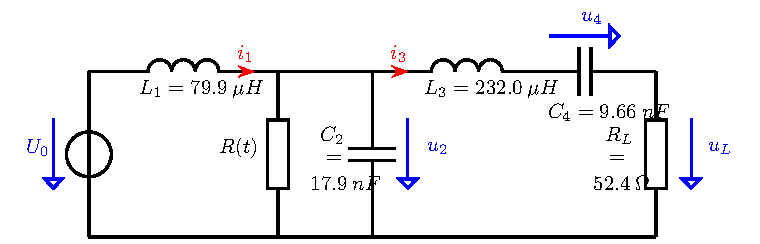
\includegraphics[width=\textwidth]{./images/ClassEAmplifier.pdf}
 % bBheightode23last5Sec.png: 1130x487 pixel, 90dpi, 31.89x13.75 cm, bb=0 0 904 390
 \caption{This is a sample image if a Class-E Amplifier.}
 \label{fig:figure}
\end{figure}
\subsection{Parametrization}
It is important to distinguish between parameters and parameter values. The latter should be specified e.g. using a parameter table such as 
Table \ref{tab:ParA}. Do not forget to explain where you got your parameter values from.
\begin{table}[!h]
{\small%
\newcommand{\mc}[3]{\multicolumn{#1}{#2}{#3}}
\begin{center}
\begin{tabular}{|c|c|c|c|c|c|c|c|c|c|c|}
 \hline
 $t_{end}$ [s] & $X_0$ [m]    & $V_0$ [m/s]  & $d$ & relTol & absTol & Refine & maxdist & Tol\\
 \hline              
      100      & $\binom{0}{2}$ & $\binom{2}{0}$ &  1  & 1e-3   &  1e-6  &    8   &     2   &  $\binom{1e-3}{1e-6}$ \\
 \hline
\end{tabular}
\end{center}
}%
\caption{Parameter set A.}
\label{tab:ParA}
\end{table}

\subsection{Implementation}

Implementation should be distinguished from the conceptual modelling (see Section \ref{sec:modelling}) and described in a separate section. Keep it brief \textbf{do not} put the whole source-code into the documentation. If there are important snippets, you may use e.g. \verb|\lstinputlisting|.

 \lstinputlisting[
 language=Matlab,
 caption={Function polar2cartesian.},
 label={SRC:polar2cartesian}]{./code/BeispielCode.m}

Listing \ref{SRC:polar2cartesian} shows the source-code of \verb|polar2cartesian| in MATLAB. 
 
Source code without file can be included via:
\begin{lstlisting}[
 basicstyle=\footnotesize, % the size of the fonts that are used for the code
 frame=single,          
 language=c++,
 numbers=left,             % where to put the line-numbers
 escapeinside={//*}{*//},  % for line labeling
 caption={Definition der Klasse \texttt{InOutputVector}.},
 label=src:InOutputVector_defs]  
 class InOutputVector:public std::vector<InOutput> {
   public:
     int untreated_entry_changes;
     
     InOutputVector() {            //* \label{lnbr:InOutput_constructor} *//
       untreated_entry_changes = 0;
     }    
     void setAt(int c,double val,double t) {
       if(true==(*this)[c].already_treated) {
         untreated_entry_changes++;
       } 
       (*this)[c].set(val,t);
     }
     double* treatAt(int c,double val) {
       if(false==(*this)[c].already_treated) {
         untreated_entry_changes--;
       }
       return((*this)[c].treat());
     }
     void treatAll() {
       for(int i=0; i<this->size(); i++){
         (*this)[i].already_treated = true;
       }
       untreated_entry_changes=0;
     }
 };
\end{lstlisting}    

In row \ref{lnbr:InOutput_constructor} in Listing \ref{src:InOutputVector_defs} we find the constructor of class
\verb|InOutputVector|.

\section{Simulation Results}
We document the results of the simulation as far as possible without potentially subjective interpretation. This is usually done with the help of plots, as in Figure \ref{fig:figure2}.
\begin{figure}[!ht]
 \centering
 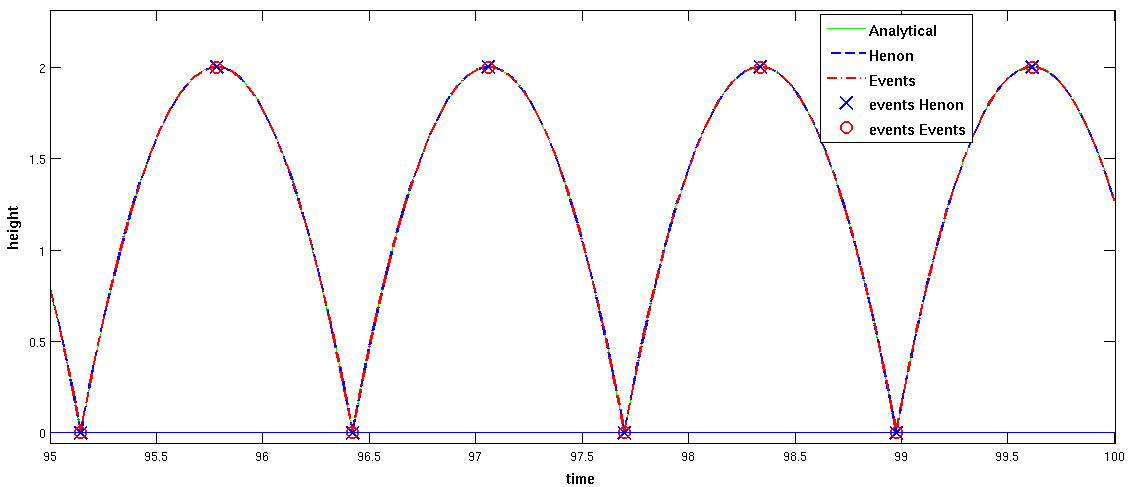
\includegraphics[width=\textwidth]{./images/bBheightode23last5Sec.png}
 % bBheightode23last5Sec.png: 1130x487 pixel, 90dpi, 31.89x13.75 cm, bb=0 0 904 390
 \caption{Simulation results when using parameter set A (see Table \ref{tab:ParA})}
 \label{fig:figure2}
\end{figure}

\section{Discussion}
\paragraph{Summary.} We tell what we told, and summarise that we showed some important \LaTeX commands for scientific writing and displayed some dummy simulation results.
\paragraph{Result Interpretation}
We interpret the results and put them in contrast with each other and the real system. 
\paragraph{Conclusion.} We conclude that writing a proper project documentation is not so hard and hope you have fun doing it yourself. 
\paragraph{Outlook.} However, we understand that further research might be necessary.
\newpage

\bibliographystyle{plain}
\bibliography{references}

\appendix
\section{Appendix}
\subsection{Not Quite Relevant Enough}
Some stuff which is not quite important enough for the main text.
\end{document}